\chapter{Quantum Physics I}
This compendium is based on MIT OpenCourseWare ``Quantum Physics I'' by Professor Allan Adams, Professor Matthew Evans, and Professor Barton Zwiebach in 2013.
I can not guarantee the accuracy of this compendium and that it is a correct interpretation of the material and explanation provided by the lecture notes and lectures. Thus, for accurate information refer to the material that this compendium is based on. If a mistake is in the compendium it is most likely my fault and not the fault of the material in which this compendium is based on.


\section{Quantum Mechanics Fundamentals}
% https://www.youtube.com/watch?v=NN2txluv1PY

Quantum Mechanics is the branch of physics that deals with the behavior of matter and energy at very small scales, typically at the level of atoms and subatomic particles. It fundamentally challenges classical mechanics by incorporating wave-particle duality, quantization of energy, and the probabilistic nature of physical systems.

Quantum mechanics has wide-ranging applications, from explaining the structure of atoms to technologies such as semiconductors and quantum computing.

\subsection{Key Concepts in Quantum Mechanics}
\begin{itemize}
    \item \textbf{Wave-Particle Duality:} Particles such as electrons exhibit both wave-like and particle-like properties. This was first demonstrated in experiments like the double-slit experiment.
    \item \textbf{Quantum State:} The state of a quantum system is described by a \textit{wavefunction}, $\psi(x,t)$, which encodes all the information about the system.
    \item \textbf{Quantization:} Physical quantities like energy and momentum are quantized, meaning they can only take discrete values.
    \item \textbf{Superposition:} A quantum system can exist in a superposition of multiple states simultaneously, with probabilities determined by the coefficients in the superposition.
    \item \textbf{Uncertainty Principle:} Formulated by Heisenberg, it states that certain pairs of physical properties, such as position and momentum, cannot both be known exactly at the same time.
\end{itemize}

\subsection{Mathematical Formulation}
The mathematical framework of quantum mechanics is built on linear algebra and functional analysis. The core equations and concepts are as follows:

\subsubsection{1. The Schrödinger Equation}
The time-dependent Schrödinger equation describes how the wavefunction evolves over time. It is given by:
\[
i\hbar \frac{\partial}{\partial t} \psi(x,t) = \hat{H} \psi(x,t)
\]
where:
\begin{itemize}
    \item $i$ is the imaginary unit.
    \item $\hbar$ is the reduced Planck's constant.
    \item $\psi(x,t)$ is the wavefunction.
    \item $\hat{H}$ is the Hamiltonian operator, which represents the total energy (kinetic + potential) of the system.
\end{itemize}

The time-independent Schrödinger equation is used for systems with no time-dependent external forces:
\[
\hat{H} \psi(x) = E \psi(x)
\]
where $E$ is the energy eigenvalue.

\subsubsection{2. Operators and Observables}
In quantum mechanics, physical observables such as position ($\hat{x}$), momentum ($\hat{p}$), and energy ($\hat{H}$) are represented by operators. These operators act on the wavefunction to extract information about the system:
\[
\hat{x} \psi(x) = x \psi(x), \quad \hat{p} = -i\hbar \frac{\partial}{\partial x}
\]
The expectation value of an observable is given by:
\[
\langle \hat{A} \rangle = \int \psi^*(x) \hat{A} \psi(x) \, dx
\]
where $\hat{A}$ is the operator corresponding to an observable.

\subsection*{3. The Heisenberg Uncertainty Principle}
The Heisenberg uncertainty principle states that it is impossible to simultaneously know the exact values of certain pairs of observables (e.g., position and momentum). Mathematically, it is expressed as:
\[
\Delta x \Delta p \geq \frac{\hbar}{2}
\]
where $\Delta x$ and $\Delta p$ are the uncertainties in position and momentum, respectively.

\subsubsection{4. The Wavefunction}
The wave function $\psi(x,t)$ contains all the information about the quantum state of a system. 
It is both injective, continues, and differentiable.
A wave function actually represents the partial, the probability amplitude. The wave function 
of a partial gives information about the behavior, both in terms of probability of position,
probability of momentum, and probability of energy. This can be a misleading interpretation
and theories are formed to give a better description of the subatomic partial. One thing 
can be determined it is not a partial in the traditional sense, e.g., a microscopic ball. 
Other interpretation, such as quantum field theory is described in section~\ref{} and provide 
a more intuitive description of what the subatomic partials actually are. However, quantum
mechanics are an abstraction that is useful.
%https://www.youtube.com/watch?v=sOI4DlWQ_1w
Its square modulus gives the probability density of finding a particle at position $x$ at time $t$:
\[
|\psi(x,t)|^2 \, dx
\]
is the probability of finding the particle in the interval $[x, x+dx]$.

For a system in a superposition of states:
\[
\psi(x,t) = \sum_{n} c_n \psi_n(x) e^{-i E_n t / \hbar}
\]
where $\psi_n(x)$ are the eigenfunctions of the Hamiltonian and $c_n$ are the coefficients determined by the initial conditions.

\subsection{Quantum Mechanics in Different Domains}
\subsubsection{1. Particle in a Box (Infinite Potential Well)}
Consider a particle confined in a one-dimensional box with infinite potential walls at $x = 0$ and $x = L$. The Schrödinger equation for this system is:
\[
\hat{H} \psi(x) = E \psi(x)
\]
with boundary conditions $\psi(0) = \psi(L) = 0$. The solutions are:
\[
\psi_n(x) = \sqrt{\frac{2}{L}} \sin \left( \frac{n\pi x}{L} \right)
\]
and the corresponding energy eigenvalues are:
\[
E_n = \frac{n^2 \pi^2 \hbar^2}{2mL^2}, \quad n = 1, 2, 3, \dots
\]

\subsubsection{2. Harmonic Oscillator}
For a quantum harmonic oscillator, the potential is given by:
\[
V(x) = \frac{1}{2} m \omega^2 x^2
\]
The energy eigenvalues for this system are quantized:
\[
E_n = \left( n + \frac{1}{2} \right) \hbar \omega
\]
and the eigenfunctions are given by Hermite polynomials.

\subsection{Quantum Entanglement and Superposition}
One of the most striking features of quantum mechanics is \textit{quantum entanglement}, where particles become correlated such that the state of one particle immediately influences the state of another, no matter the distance separating them. This leads to phenomena such as:
\begin{itemize}
    \item \textbf{Non-locality:} The measurement of one particle's state can instantaneously affect the state of another.
    \item \textbf{Bell's Theorem:} A set of inequalities that show that no local hidden variable theory can explain quantum correlations.
\end{itemize}


%\subsection{Applications of Quantum Mechanics}
%Quantum mechanics is fundamental to many modern technologies and fields, including:
%\begin{itemize}
%    \item \textbf{Semiconductors:} Quantum mechanics is essential in the design of transistors and other semiconductor devices.
%    \item \textbf{Quantum Computing:} Quantum computers exploit quantum superposition and entanglement to perform calculations exponentially faster than classical computers.
%    \item \textbf{Quantum Cryptography:} Uses principles of quantum mechanics, such as the no-cloning theorem, to secure communication.
%    \item \textbf{Nuclear Magnetic Resonance (NMR) and MRI:} Quantum mechanical principles are applied in these imaging techniques.
%\end{itemize}
%
%\subsection{Conclusion}
%Quantum mechanics represents a profound shift from classical mechanics, incorporating a probabilistic and wave-like nature to the behavior of particles. It forms the basis for much of modern physics, with applications in a wide range of technologies. The theory continues to evolve, with new interpretations and extensions, such as quantum field theory and quantum gravity, exploring the interplay between quantum mechanics and general relativity.


\section{Quantum Field Theory}
%https://www.youtube.com/watch?v=xQFgk-nEihg&list=PLUl4u3cNGP61AV6bhf4mB3tCyWQrI_uU5
Quantum Field Theory (QFT) is the theoretical framework that combines quantum mechanics and special relativity to describe the fundamental interactions of particles through fields. In QFT, particles are excitations of underlying quantum fields, and their interactions are mediated by the exchange of field quanta.

\subsection{Core Principles of QFT}
\begin{enumerate}
    \item \textbf{Field Quantization:} Classical fields, such as the electromagnetic field, are quantized to produce quantum fields. Each field corresponds to a particle type. For instance:
    \begin{itemize}
        \item The electromagnetic field corresponds to photons.
        \item The electron field corresponds to electrons.
    \end{itemize}

    \item \textbf{Wave-Particle Duality:} Particles exhibit both wave-like and particle-like behavior. Fields describe the wave aspect, while excitations of the fields (quanta) represent particles.

    \item \textbf{Lagrangian Formulation:} The dynamics of quantum fields are determined by a Lagrangian density \(\mathcal{L}\), which encodes the symmetries and interactions of the system.
    
    \item \textbf{Symmetry and Conservation Laws:} The symmetries of the Lagrangian, via Noether's theorem, lead to conservation laws. For example:
    \begin{itemize}
        \item Translational symmetry \(\rightarrow\) conservation of momentum.
        \item Rotational symmetry \(\rightarrow\) conservation of angular momentum.
        \item Gauge symmetry \(\rightarrow\) conservation of charge.
    \end{itemize}

    \item \textbf{Interactions and Feynman Diagrams:} Interactions between particles are described by terms in the Lagrangian. These interactions can be visualized and computed using Feynman diagrams.
\end{enumerate}

\subsection{Principle of locality}
Any field $a$ is denoted as $\phi_a(\overline{x},t)$.

The action $S$, i.e., how fields moves or changes in a physical system.
\begin{equation*}
    S = \int \mathcal{L}(\phi_a(x), \partial_\mu \phi_a(x)) \, d^4x
\end{equation*}
also known as local form where the action is expressed as an integral over a local density, i.e., the Lagrangian density.
The $d^4x$ term is the infinitesimal volume element in spacetime, i.e., $d^4x=dtdxdydz$.
The $\partial_\mu \phi_a(x)$ term is the derivatives of the field(s).


The momentum density $\Pi$, i.e., how the momentum is distributed across space.
\begin{eqnarray*}
    \Pi_a(\overline{x},t) = \frac{\partial \mathcal{L}}{\partial \phi_a(\overline{x},t)}
\end{eqnarray*}

Hamiltonian $\mathcal{H}$

\subsection{Mathematical Framework}
\subsubsection{Lagrangian Density}
The Lagrangian density \(\mathcal{L}\) governs the behavior of a field \(\phi(x)\). For a free scalar field, it is given by:
\[
\mathcal{L} = \frac{1}{2} \partial^\mu \phi \partial_\mu \phi - \frac{1}{2}m^2\phi^2,
\]
where \(\partial^\mu = \frac{\partial}{\partial x_\mu}\) is the spacetime derivative, and \(m\) is the mass of the field quanta.

\subsubsection{Quantization}
Field quantization replaces classical fields with operators. For a scalar field \(\phi(x)\):
\[
\phi(x) = \int \frac{d^3k}{(2\pi)^3} \frac{1}{\sqrt{2\omega_k}} \Big( a_k e^{-i k \cdot x} + a_k^\dagger e^{i k \cdot x} \Big),
\]
where:
\begin{itemize}
    \item \(a_k\) and \(a_k^\dagger\) are annihilation and creation operators.
    \item \(\omega_k = \sqrt{\vec{k}^2 + m^2}\) is the energy.
\end{itemize}

\subsubsection{Propagators}
Propagators describe how particles move through spacetime. For a scalar field, the propagator is:
\[
D_F(x - y) = \int \frac{d^4k}{(2\pi)^4} \frac{e^{-i k \cdot (x - y)}}{k^2 - m^2 + i\epsilon}.
\]

\subsubsection{Interactions}
Interactions are introduced by adding terms to the Lagrangian. For example, for a scalar field with quartic interaction:
\[
\mathcal{L} = \frac{1}{2} \partial^\mu \phi \partial_\mu \phi - \frac{1}{2}m^2\phi^2 - \frac{\lambda}{4!}\phi^4,
\]
where \(\lambda\) is the coupling constant.


%\subsection{The Principle of Locality}
%In field theories such as classical field theory and quantum field theory, the principle of locality can be stated as follows:
%
%\begin{quote}
%\textit{Physical interactions occur only at points that are infinitesimally close in spacetime. Information or causal influence cannot propagate faster than the speed of light, $c$.}
%\end{quote}
%
%\subsubsection{Local Commutativity (or Microcausality)}
%
%In quantum field theory, locality is encapsulated in the condition of \textbf{microcausality}, which states that the field operators commute (or anticommute for fermionic fields) at spacelike separations:
%\[
%\left[ \hat{\phi}(x), \hat{\phi}(y) \right] = 0, \quad \text{for } (x-y)^2 < 0.
%\]
%Here:
%\begin{itemize}
%    \item $\hat{\phi}(x)$ is the field operator at spacetime point $x$.
%    \item $(x-y)^2 = (t_x - t_y)^2 - |\mathbf{x} - \mathbf{y}|^2$ is the spacetime interval.
%    \item The condition $(x-y)^2 < 0$ ensures that the separation is spacelike.
%\end{itemize}
%
%This ensures that no information or causal influence can propagate between $x$ and $y$, as spacelike separations imply events are outside each other's light cones.
%
%\subsubsection{Local Action Principle}
%
%The principle of locality is also reflected in the action functional of field theories. The action $S$ is a local integral over a Lagrangian density $\mathcal{L}$, which depends only on the fields and their derivatives at a given point:
%\[
%S = \int \mathcal{L}(\phi, \partial_\mu \phi) \, d^4x.
%\]
%
%The Lagrangian density $\mathcal{L}$ encodes the dynamics of the field $\phi$, and locality demands that $\mathcal{L}$ at a spacetime point $x$ does not depend on the fields at other points.
%
%\subsubsection{Relativistic Causality}
%
%Relativistic causality is preserved by requiring that the commutators of observable quantities vanish outside the light cone:
%\[
%\left[ \hat{\mathcal{O}}(x), \hat{\mathcal{O}}(y) \right] = 0, \quad \text{if } (x-y)^2 < 0.
%\]
%This ensures that measurements made at spacelike-separated points do not influence each other, maintaining locality.
%
%\subsubsection{Nonlocal Phenomena in Quantum Mechanics}
%
%While locality holds in classical field theory and quantum field theory under relativistic conditions, certain quantum phenomena, such as entanglement, challenge the classical notion of locality. For example, Bell's theorem demonstrates that quantum correlations violate local hidden variable theories, though this does not allow faster-than-light communication.


\subsection{Renormalization}
\begin{itemize}
    \item \textbf{Problem:} Quantum field calculations often produce infinities.
    \item \textbf{Solution:} Renormalization systematically removes these infinities by redefining parameters (e.g., mass, charge) in the theory.
\end{itemize}

\subsection{Applications of QFT}
\begin{enumerate}
    \item \textbf{Standard Model of Particle Physics:} Describes electromagnetic, weak, and strong interactions using gauge theories (e.g., Quantum Electrodynamics, Quantum Chromodynamics).
    \item \textbf{Condensed Matter Physics:} Explains phenomena such as superconductivity and quantum phase transitions.
    \item \textbf{Cosmology:} Provides insight into early-universe phenomena like inflation and dark matter.
\end{enumerate}



\section{The Standard Model of Subatomic Particles}
The Standard Model categorizes particles into \textit{fermions} and \textit{bosons}:
\begin{itemize}
    \item \textbf{Fermions:} These are the building blocks of matter. They obey the Pauli Exclusion Principle and are divided into two families:
    \begin{itemize}
        \item \textit{Quarks:} Six types (flavors) of quarks: \textbf{up (u), down (d), charm (c), strange (s), top (t), and bottom (b)}. Quarks combine to form hadrons, such as protons and neutrons.
        \item \textit{Leptons:} Six types of leptons, including the electron $(e^-)$, muon $(\mu^-)$, tau $(\tau^-)$, and their associated neutrinos $(\nu_e, \nu_\mu, \nu_\tau)$.
    \end{itemize}
    \item \textbf{Bosons:} These are force carriers, mediating the fundamental interactions:
    \begin{itemize}
        \item \textit{Photon ($\gamma$):} Mediates the electromagnetic force.
        \item \textit{W$^\pm$, Z$^0$:} Mediate the weak nuclear force.
        \item \textit{Gluon ($g$):} Mediates the strong nuclear force.
        \item \textit{Higgs Boson ($H$):} Provides mass to particles through the Higgs mechanism.
    \end{itemize}
\end{itemize}

\begin{figure}[H]
   \centering 
  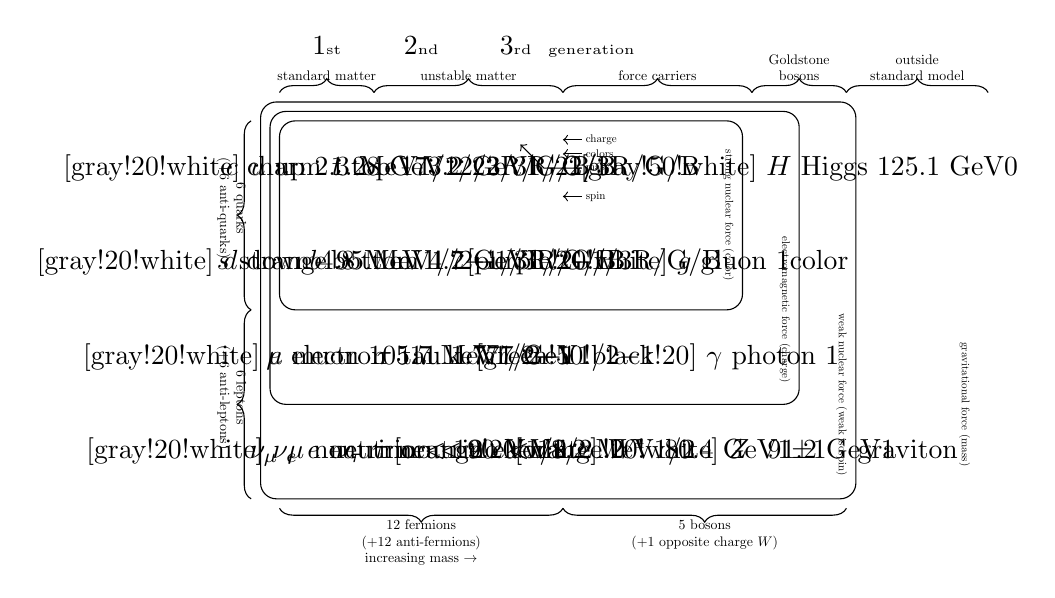
\begin{tikzpicture}[
      brace/.style = { decorate, decoration={brace, amplitude=5pt} },
      mbrace/.style = { decorate, decoration={brace, amplitude=5pt, mirror} },
      label/.style = { black, midway, scale=0.5, align=center },
      toplabel/.style = { label, above=.5em, anchor=south },
      leftlabel/.style = { label,rotate=-90,left=.5em,anchor=north },   
      bottomlabel/.style = { label, below=.5em, anchor=north },
      force/.style = { rotate=-90,scale=0.4 },
      round/.style = { rounded corners=2mm },
      legend/.style = { right,scale=0.4 },
      nosep/.style = { inner sep=0pt },
      generation/.style = { anchor=base },
      x=1.2cm, y=1.2cm,
    ]
    \draw[round] (-0.5,0.5) rectangle (4.4,-1.5);
    \draw[round] (-0.6,0.6) rectangle (5.0,-2.5);
    \draw[round] (-0.7,0.7) rectangle (5.6,-3.5);
  
    \node at(0, 0)   {\particle[gray!20!white]
                     {$u$}        {up}       {$2.3$ MeV}{1/2}{$2/3$}{R/G/B}};
    \node at(0,-1)   {\particle[gray!20!white]
                     {$d$}        {down}    {$4.8$ MeV}{1/2}{$-1/3$}{R/G/B}};
    \node at(0,-2)   {\particle[gray!20!white]
                     {$e$}        {electron}       {$511$ keV}{1/2}{$-1$}{}};
    \node at(0,-3)   {\particle[gray!20!white]
                     {$\nu_e$}    {$e$ neutrino}         {$<2$ eV}{1/2}{}{}};
    \node at(1, 0)   {\particle
                     {$c$}        {charm}   {$1.28$ GeV}{1/2}{$2/3$}{R/G/B}};
    \node at(1,-1)   {\particle 
                     {$s$}        {strange}  {$95$ MeV}{1/2}{$-1/3$}{R/G/B}};
    \node at(1,-2)   {\particle
                     {$\mu$}      {muon}         {$105.7$ MeV}{1/2}{$-1$}{}};
    \node at(1,-3)   {\particle
                     {$\nu_\mu$}  {$\mu$ neutrino}    {$<190$ keV}{1/2}{}{}};
    \node at(2, 0)   {\particle
                     {$t$}        {top}    {$173.2$ GeV}{1/2}{$2/3$}{R/G/B}};
    \node at(2,-1)   {\particle
                     {$b$}        {bottom}  {$4.7$ GeV}{1/2}{$-1/3$}{R/G/B}};
    \node at(2,-2)   {\particle
                     {$\tau$}     {tau}          {$1.777$ GeV}{1/2}{$-1$}{}};
    \node at(2,-3)   {\particle
                     {$\nu_\tau$} {$\tau$ neutrino}  {$<18.2$ MeV}{1/2}{}{}};
    \node at(3,-3)   {\particle[orange!20!white]
                     {$W^{\hspace{-.3ex}\scalebox{.5}{$\pm$}}$}
                                  {}              {$80.4$ GeV}{1}{$\pm1$}{}};
    \node at(4,-3)   {\particle[orange!20!white]
                     {$Z$}        {}                    {$91.2$ GeV}{1}{}{}};
    \node at(3.5,-2) {\particle[green!50!black!20]
                     {$\gamma$}   {photon}                        {}{1}{}{}};
    \node at(3.5,-1) {\particle[purple!20!white]
                     {$g$}        {gluon}                    {}{1}{}{color}};
    \node at(5,0)    {\particle[gray!50!white]
                     {$H$}        {Higgs}              {$125.1$ GeV}{0}{}{}};
    \node at(6.1,-3) {\particle
                     {}           {graviton}                       {}{}{}{}};
  
    \node at(4.25,-0.5) [force]      {strong nuclear force (color)};
    \node at(4.85,-1.5) [force]    {electromagnetic force (charge)};
    \node at(5.45,-2.4) [force] {weak nuclear force (weak isospin)};
    \node at(6.75,-2.5) [force]        {gravitational force (mass)};
  
    \draw [<-] (2.5,0.3)   -- (2.7,0.3)          node [legend] {charge};
    \draw [<-] (2.5,0.15)  -- (2.7,0.15)         node [legend] {colors};
    \draw [<-] (2.05,0.25) -- (2.3,0) -- (2.7,0) node [legend]   {mass};
    \draw [<-] (2.5,-0.3)  -- (2.7,-0.3)         node [legend]   {spin};
  
    \draw [mbrace] (-0.8,0.5)  -- (-0.8,-1.5)
                   node[leftlabel] {6 quarks\\(+6 anti-quarks)};
    \draw [mbrace] (-0.8,-1.5) -- (-0.8,-3.5)
                   node[leftlabel] {6 leptons\\(+6 anti-leptons)};
    \draw [mbrace] (-0.5,-3.6) -- (2.5,-3.6)
                   node[bottomlabel]
                   {12 fermions\\(+12 anti-fermions)\\increasing mass $\to$};
    \draw [mbrace] (2.5,-3.6) -- (5.5,-3.6)
                   node[bottomlabel] {5 bosons\\(+1 opposite charge $W$)};
  
    \draw [brace] (-0.5,.8) -- (0.5,.8) node[toplabel]         {standard matter};
    \draw [brace] (0.5,.8)  -- (2.5,.8) node[toplabel]         {unstable matter};
    \draw [brace] (2.5,.8)  -- (4.5,.8) node[toplabel]          {force carriers};
    \draw [brace] (4.5,.8)  -- (5.5,.8) node[toplabel]       {Goldstone\\bosons};
    \draw [brace] (5.5,.8)  -- (7,.8)   node[toplabel] {outside\\standard model};
  
    \node at (0,1.2)   [generation] {1\tiny st};
    \node at (1,1.2)   [generation] {2\tiny nd};
    \node at (2,1.2)   [generation] {3\tiny rd};
    \node at (2.8,1.2) [generation] {\tiny generation};
  \end{tikzpicture}
  \caption{This improved diagram of the standard model of physics was made at the CERN Webfest 2012 by David Galbraith and Carsten Burgard.}
  %https://texample.net/model-physics/
\end{figure}


\subsection{Fundamental Forces}
The Standard Model describes three forces:
\begin{itemize}
    \item \textbf{Electromagnetic Force:} Described by Quantum Electrodynamics (QED). It is mediated by photons and affects particles with electric charge.
    \item \textbf{Weak Nuclear Force:} Responsible for processes like beta decay. It is mediated by W$^\pm$ and Z$^0$ bosons and affects all fermions.
    \item \textbf{Strong Nuclear Force:} Described by Quantum Chromodynamics (QCD). It binds quarks together into hadrons and is mediated by gluons.
\end{itemize}

The fourth fundamental force, gravity, is not included in the Standard Model but is described separately by General Relativity.


\subsection{Mathematical Framework}
The Standard Model is based on the principles of quantum field theory (QFT), which combines quantum mechanics and special relativity. The fields and their interactions are described using the following components:

\subsubsection{1. Lagrangian of the Standard Model}
The dynamics of particles in the Standard Model are encoded in the Lagrangian, which is a function of the fields and their derivatives:
\[
\mathcal{L} = \mathcal{L}_{\text{gauge}} + \mathcal{L}_{\text{fermion}} + \mathcal{L}_{\text{Higgs}}
\]
\begin{itemize}
    \item $\mathcal{L}_{\text{gauge}}$: Describes the interactions of gauge fields (force carriers).
    \item $\mathcal{L}_{\text{fermion}}$: Describes the dynamics of fermions.
    \item $\mathcal{L}_{\text{Higgs}}$: Describes the Higgs field and its interactions.
\end{itemize}

\subsubsection{2. Gauge Symmetries}
The Standard Model is built on the symmetry group:
\[
SU(3)_C \times SU(2)_L \times U(1)_Y
\]
where:
\begin{itemize}
    \item $SU(3)_C$: Describes the strong interaction (QCD).
    \item $SU(2)_L \times U(1)_Y$: Describes the electroweak interaction.
\end{itemize}

\subsubsection{3. Higgs Mechanism}
The Higgs mechanism explains how particles acquire mass. The Higgs field, $\phi$, interacts with particles, and its nonzero vacuum expectation value breaks the electroweak symmetry, giving mass to W$^\pm$, Z$^0$, and fermions:
\[
m = g \, v
\]
where $g$ is the coupling constant, and $v$ is the vacuum expectation value of the Higgs field.


\section{Electromagnetic Waves}
\subsection{Introduction}
Electromagnetic waves are a fundamental aspect of both classical and quantum physics. While classical physics describes them as oscillating electric and magnetic fields propagating through space, quantum physics provides a deeper understanding by describing them in terms of quantum electrodynamics (QED) and photons. In this framework:
\begin{itemize}
    \item Electromagnetic waves are quantized.
    \item The wave-particle duality explains the dual behavior of electromagnetic radiation.
    \item Photons are the quantum carriers of electromagnetic interactions.
\end{itemize}

This document provides a detailed summary of electromagnetic waves from the perspective of quantum physics.

\subsection{Wave-Particle Duality}
Quantum physics posits that electromagnetic waves exhibit both particle-like and wave-like properties:
\begin{itemize}
    \item \textbf{Wave-like behavior:} Electromagnetic waves are described by the Maxwell equations in their classical form. The electric field $\vec{E}$ and the magnetic field $\vec{B}$ oscillate perpendicular to each other and the direction of propagation.
    \item \textbf{Particle-like behavior:} The quantization of electromagnetic waves leads to the concept of the \textit{photon}, the fundamental quantum of light.
\end{itemize}

Mathematically, the energy $E$ and momentum $p$ of a photon are related to the frequency $\nu$ and wavelength $\lambda$ of the wave as:
\[
E = h \nu, \quad p = \frac{h}{\lambda},
\]
where $h$ is Planck's constant.

\subsection*{Quantization of the Electromagnetic Field}
The quantization of electromagnetic waves is described by quantum electrodynamics (QED). The electric and magnetic fields are treated as operators acting on a quantum state.

\subsubsection{Classical Fields and Quantization}
In classical physics, the electromagnetic wave can be described as:
\[
\vec{E}(\vec{r}, t) = \vec{E}_0 \cos(\vec{k} \cdot \vec{r} - \omega t),
\quad
\vec{B}(\vec{r}, t) = \vec{B}_0 \cos(\vec{k} \cdot \vec{r} - \omega t),
\]
where:
\begin{itemize}
    \item $\vec{E}_0$ and $\vec{B}_0$ are the amplitudes of the electric and magnetic fields.
    \item $\vec{k}$ is the wave vector.
    \item $\omega$ is the angular frequency.
\end{itemize}

In quantum physics, these fields are replaced by operators:
\[
\hat{\vec{E}}(\vec{r}, t), \quad \hat{\vec{B}}(\vec{r}, t),
\]
which act on the quantum state of the electromagnetic field.

\subsubsection{Photon Creation and Annihilation Operators}
The quantized electromagnetic field is expressed in terms of photon creation and annihilation operators:
\[
\hat{A}^\dagger(\vec{k}) \quad \text{(creation operator)},
\quad
\hat{A}(\vec{k}) \quad \text{(annihilation operator)},
\]
which satisfy the commutation relation:
\[
[\hat{A}(\vec{k}), \hat{A}^\dagger(\vec{k}')] = \delta^3(\vec{k} - \vec{k}').
\]

The quantized electric field operator, for example, is written as:
\[
\hat{\vec{E}}(\vec{r}, t) = i \sum_{\vec{k}, \lambda} \sqrt{\frac{\hbar \omega_k}{2 \epsilon_0 V}}
\left[
\hat{A}(\vec{k}, \lambda) \vec{\epsilon}(\lambda) e^{i (\vec{k} \cdot \vec{r} - \omega_k t)} 
- \hat{A}^\dagger(\vec{k}, \lambda) \vec{\epsilon}^*(\lambda) e^{-i (\vec{k} \cdot \vec{r} - \omega_k t)}
\right],
\]
where:
\begin{itemize}
    \item $\lambda$ denotes the polarization state of the photon.
    \item $\vec{\epsilon}(\lambda)$ is the polarization vector.
    \item $\omega_k = c |\vec{k}|$ is the angular frequency.
    \item $V$ is the quantization volume.
\end{itemize}

\subsection{Interaction with Matter}
Photons interact with matter through processes such as:
\begin{itemize}
    \item \textbf{Absorption:} A photon is absorbed by an atom, raising an electron to a higher energy level.
    \item \textbf{Emission:} An atom releases a photon when an electron transitions to a lower energy level.
    \item \textbf{Scattering:} Photons interact with charged particles, changing their direction and energy.
\end{itemize}

The probability of these interactions is described by the **transition amplitude**, which is calculated using Feynman diagrams in QED.

\subsubsection{Absorption and Emission}
The energy difference $\Delta E$ between two atomic levels determines the frequency of the absorbed or emitted photon:
\[
\hbar \omega = \Delta E.
\]

\subsubsection{Scattering Processes}
In Compton scattering, for example, a photon scatters off an electron, transferring energy and momentum:
\[
\lambda' - \lambda = \frac{h}{m_e c} (1 - \cos \theta),
\]
where $\lambda$ and $\lambda'$ are the wavelengths before and after scattering, $m_e$ is the electron mass, and $\theta$ is the scattering angle.

\subsection{Coherence and Quantum Superposition}
Electromagnetic waves can exhibit quantum coherence, where the wavefunction of the photon is a superposition of states:
\[
\ket{\psi} = c_1 \ket{E_1} + c_2 \ket{E_2},
\]
where $c_1$ and $c_2$ are complex coefficients. This principle underlies phenomena such as:
\begin{itemize}
    \item \textbf{Interference:} When photons combine constructively or destructively.
    \item \textbf{Entanglement:} When two photons share correlated quantum states.
\end{itemize}

\subsection{Experimental Evidence}
Quantum properties of electromagnetic waves have been verified through experiments such as:
\begin{itemize}
    \item \textbf{Photoelectric Effect:} Demonstrates the particle nature of light.
    \item \textbf{Double-Slit Experiment:} Shows wave-particle duality.
    \item \textbf{Quantum Electrodynamics (QED):} Accurately predicts phenomena like the Lamb shift and anomalous magnetic moment of the electron.
\end{itemize}

\subsection{Conclusion}
In quantum physics, electromagnetic waves are understood as quantized fields composed of photons, which exhibit both wave-like and particle-like behavior. Quantum electrodynamics provides a robust framework for describing their interactions with matter and their fundamental properties. This dual nature of electromagnetic waves is at the heart of modern physics and has profound implications for both theoretical understanding and technological applications.

% Entropy, it is more likely that a hot object obmits the eat as energy wants to diapate but it is posible the "movment/vibration" stais within the object and the serounding vibration affects the object making it hotter than it initialy was.
% heat diapation, heat cotains more vibrations and natuarly want to spread out which is why heat moves from hot to could. Why a room gets colder is the los in heat to the cold source.
% this is for instance why it fels colder close to a window on a cold day. This affect can be faster if the hold air is forced with a fan or other forms that causes air flow.
% air flow is a macroscopic affect where the slow vibrating atoms and molocules are spread out into higher vibrating space, casing more cold surface area, i.e., faster heat disapating. in other words you move the automs and molicules but causes very litle increase in vibration which is heat. One form of energy

% Entorpy might be the cause of life, since it is life causes increase in entropy

% standard model of elementary particles
% Dark matter and dark energy could potentialy be described as an extension of the standard model
% Where bare particles and vertial particals anrth real particles just mathematical model to describe quantom effects

%https://www.youtube.com/watch?v=Zkv8sW6y3sY



\section{Electricity}

\section{Mass}
% Higgs field
% SU(2) 
% Lie algebra
% https://www.youtube.com/watch?v=wiBsfvW5AWY&t=542s
% m = E/c^2

\section{General relativity}
General relativity (GR) is a theory of gravitation proposed by Albert Einstein in 1915. It extends the principle of relativity and incorporates the equivalence principle, providing a unified description of gravity as the curvature of spacetime caused by mass and energy.
General relativity is not a quantum effect in they way it is defined, however, it is generalized version of special relativity which is related to QFT.
One of the big unsolved questions is the combination gravity with quantum physics into a unified theory of 
every thing. Many theories have been developed, but none has been proven. 
%Why general relativity is summaries in this chapter it also dues to the concept of spacetime.


\subsection{Core Concepts}

\subsubsection{Principle of Equivalence}
The equivalence principle states that the effects of gravity are locally indistinguishable from acceleration. This principle laid the foundation for the geometric interpretation of gravity.

\subsubsection{Spacetime and the Metric Tensor}
Spacetime is a four-dimensional continuum that combines space and time. The geometry of spacetime is described by the metric tensor $g_{\mu \nu}$, which encodes the distances between events in spacetime:
\[
\mathrm{d}s^2 = g_{\mu \nu} \mathrm{d}x^{\mu} \mathrm{d}x^{\nu},
\]
where $\mathrm{d}s^2$ is the spacetime interval, and $\mathrm{d}x^{\mu}$ and $\mathrm{d}x^{\nu}$ are infinitesimal displacements in spacetime coordinates.

\subsubsection{Einstein Field Equations (EFE)}
The Einstein field equations describe how matter and energy determine the curvature of spacetime:
\[
R_{\mu \nu} - \frac{1}{2} g_{\mu \nu} R + \Lambda g_{\mu \nu} = \frac{8 \pi G}{c^4} T_{\mu \nu},
\]
where:
\begin{itemize}
  \item $R_{\mu \nu}$ is the Ricci curvature tensor,
  \item $R$ is the Ricci scalar,
  \item $g_{\mu \nu}$ is the metric tensor,
  \item $\Lambda$ is the cosmological constant,
  \item $T_{\mu \nu}$ is the stress-energy tensor,
  \item $G$ is the gravitational constant,
  \item $c$ is the speed of light.
\end{itemize}

\subsubsection{Geodesics}
Objects in free fall follow geodesics, which are the straightest possible paths in curved spacetime. The geodesic equation is given by:
\[
\frac{\mathrm{d}^2 x^{\mu}}{\mathrm{d}\tau^2} + \Gamma^{\mu}_{\nu \lambda} \frac{\mathrm{d}x^{\nu}}{\mathrm{d}\tau} \frac{\mathrm{d}x^{\lambda}}{\mathrm{d}\tau} = 0,
\]
where $\Gamma^{\mu}_{\nu \lambda}$ are the Christoffel symbols, representing the connection coefficients of spacetime.


\subsection{Key Predictions}

\subsubsection{Gravitational Time Dilation}
Time runs slower in stronger gravitational fields. This effect has been confirmed through experiments such as the Pound-Rebka experiment and GPS satellite systems.

\subsubsection{Gravitational Redshift}
Light emitted from a strong gravitational field is redshifted due to the loss of energy as it escapes the field.

\subsubsection{Bending of Light (Gravitational Lensing)}
Light rays passing near a massive object are bent due to spacetime curvature. This effect has been confirmed by observations of stars near the Sun during a solar eclipse.

\subsubsection{Black Holes}
Solutions to the Einstein field equations, such as the Schwarzschild solution, predict the existence of black holes, regions of spacetime where gravity is so strong that not even light can escape.

\subsubsection{Gravitational Waves}
Ripples in spacetime caused by accelerating massive objects, predicted by GR and confirmed by LIGO's detection in 2015.

\subsection{Mathematical Framework}

\subsubsection{Metric Tensor and Curvature}
The curvature of spacetime is described by the Riemann curvature tensor $R^{\rho}_{\sigma \mu \nu}$, which is derived from the metric tensor $g_{\mu \nu}$ and its derivatives.

\subsubsection{Stress-Energy Tensor}
The stress-energy tensor $T_{\mu \nu}$ describes the distribution of matter and energy in spacetime, including density, momentum, and pressure.

\subsubsection{Cosmological Constant}
The cosmological constant $\Lambda$ represents the energy density of empty space (vacuum energy) and plays a key role in cosmology, particularly in the accelerated expansion of the universe.

\subsection{Applications and Observations}

\subsubsection{Cosmology}
GR is the foundation of modern cosmology, explaining the dynamics of the universe, the Big Bang, and cosmic inflation.

\subsubsection{Astrophysics}
GR is essential for understanding black holes, neutron stars, and gravitational wave phenomena.

\subsubsection{Technology}
Applications such as GPS rely on corrections from GR to account for time dilation and spacetime curvature.


% https://www.youtube.com/watch?v=qsNQneMxYiQ
% Lorentz transformations
% Schwarzschild radius

% Dark energy and dark matter
% https://www.youtube.com/watch?v=YNEBhwimJWs&t=27s

% Cosmology
% bubble universes
% ekpyrotic model
% cyclic model
% Loop quantum gravity
% Lattice Field Theory https://www.youtube.com/watch?v=_1HJi4qn-xo

